\documentclass{standalone}
\usepackage{tikz}
\usepackage{ctex,siunitx}
\setCJKmainfont{Noto Serif CJK SC}
\usepackage{tkz-euclide}
\usepackage{amsmath}
\usetikzlibrary{patterns, calc,3d}
\usetikzlibrary {decorations.pathmorphing,decorations.pathreplacing,decorations.shapes,}
\begin{document}
\small
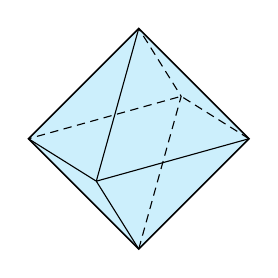
\begin{tikzpicture}[>=latex,scale=1.4]
  % \useasboundingbox(-1.0,-1.4)rectangle(3.5,3.7);
  \draw[fill=cyan!20,semithick](0,1,0)--(-1,0,0)--(0,-1,0)--(1,0,0)--cycle;
  \draw[thin](1,0,0)--(0,0,1)--(-1,0,0)(0,-1,0)--(0,0,1)--(0,1,0);
  \draw[thin,densely dashed](1,0,0)--(0,0,-1)--(-1,0,0)(0,-1,0)--(0,0,-1)--(0,1,0);
\end{tikzpicture}
\end{document}